\documentclass{article}
\usepackage[magyar]{babel}
\usepackage{t1enc}
\usepackage{graphicx}
\usepackage{amsmath}
\usepackage[export]{adjustbox}
\graphicspath{ {./images/} }

\title{Ohm és Kirchoff törvényei}
\author{Bejó Dávid}
\date{2024}

\begin{document}

\maketitle

\section{Bevezetés}
Az Ohm-törvény és a Kirchhoff-törvények az elektrotechnika és a fizika területén alapvető elvek, amelyek alapvető keretet biztosítanak az elektromos áramkörök megértéséhez és elemzéséhez. Ezek a törvények képezik az áramkörelmélet sarokkövét, lehetővé téve a mérnökök és a tudósok számára az elektromos rendszerek előrejelzését, tervezését és hibaelhárítását.

\section{Ohm törvénye}
Ha két változó mennyiség hányadosa állandó, akkor azt mondjuk, hogy a két mennyiség egyenesen arányos. A fogyasztóra kapcsolt feszültség egyenesen arányos a fogyasztón átfolyó áram erősségével. Ez Ohm törvénye. Nevét felfedezőjéről, Georg Simon Ohm (1787–1854) német fizikusról kapta. Róla nevezték el az elektromos ellenállás mértékegységét. Ohm törvényének alapegyenlete a következő:
\begin{equation}
    U = I \cdot R
\end{equation}
ahol:
\begin{itemize}
    \item $U$ a fogyasztón mért feszültséget jelenti voltban (V),
    \item $I$ a fogyasztón átfolyó áram amperben kifejezve (A),
    \item $R$ a fogyasztó ellenállása ohmban ($\Omega$).
\end{itemize}

\section{Feszültség, áramerősség és ellenállás}
\subsection{Feszültség (\textit{V})}
A feszültség megmutatja, hogy mennyi munkát végez az elektromos mező, miközben 1 C töltést a mező egyik pontjából a másikba áramoltat.

\subsection{Áramerősség (\textit{I})}
Az áramerősség megmutatja, hogy mekkora a vezető keresztmetszetén 1 s alatt átáramlott elektromos tulajdonságú részecskék együttes töltése.

\subsection{Ellenállás (\textit{R})}
A fogyasztóknak azt a tulajdonságát, hogy anyaguk részecskéi akadályozzák az elektromos tulajdonságú részecskék áramlását.

\section{Ohm törvénye soros és párhuzamos kapcsolásokban}

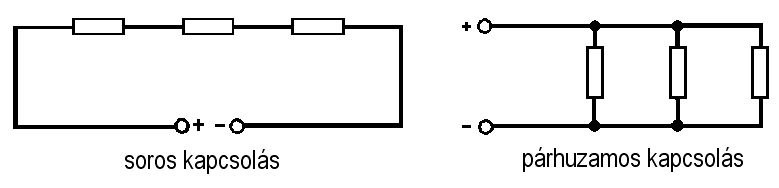
\includegraphics[width=\textwidth]{kapcsolasok}

\subsection{Soros kapcsolás}
Ha két ellenállásnak csak az egyik vége van összekötve, és közéjük semmi más nem kapcsolódik, akkor a két elem sorba van kapcsolva. A sorosan kapcsolt ellenállások összege egyenlő az eredő ellenállás ($R_{\text{eredő}}$) összegével:
\begin{equation}
    R_{\text{eredő}} = R_1 + R_2 + \ldots + R_n
\end{equation}

\subsection{Párhuzamos kapcsolás}
Párhuzamos kapcsolásnak azt nevezzük, amikor az alkatrészek azonos végüknél vannak összekötve.
Az eredő ellenállás reciproka egyenlő a párhuzamosan kapcsolt ellenállások reciprokainak összegével:
\begin{equation}
    \frac{1}{R_{\text{eredő}}} = \frac{1}{R_1} + \frac{1}{R_2} + \ldots + \frac{1}{R_n}
\end{equation}
\pagebreak
\section{Kirchhoff-törvények}
A Kirchhoff-törvények a villamosságtanban a töltés és az energia megmaradását tárgyalják. Először Gustav Kirchhoff (1824-1887) mondta ki őket 1845-ben. 

\section{Kirchhoff I. törvénye: a csomóponti törvény}
Kirchhoff csomóponti törvénye szerint a csomópontba befolyó áramok összege megyegyezik a csomópontból kifolyó áramok összegével, azaz a csomópont áramainak előjelhelyes összege nulla. 

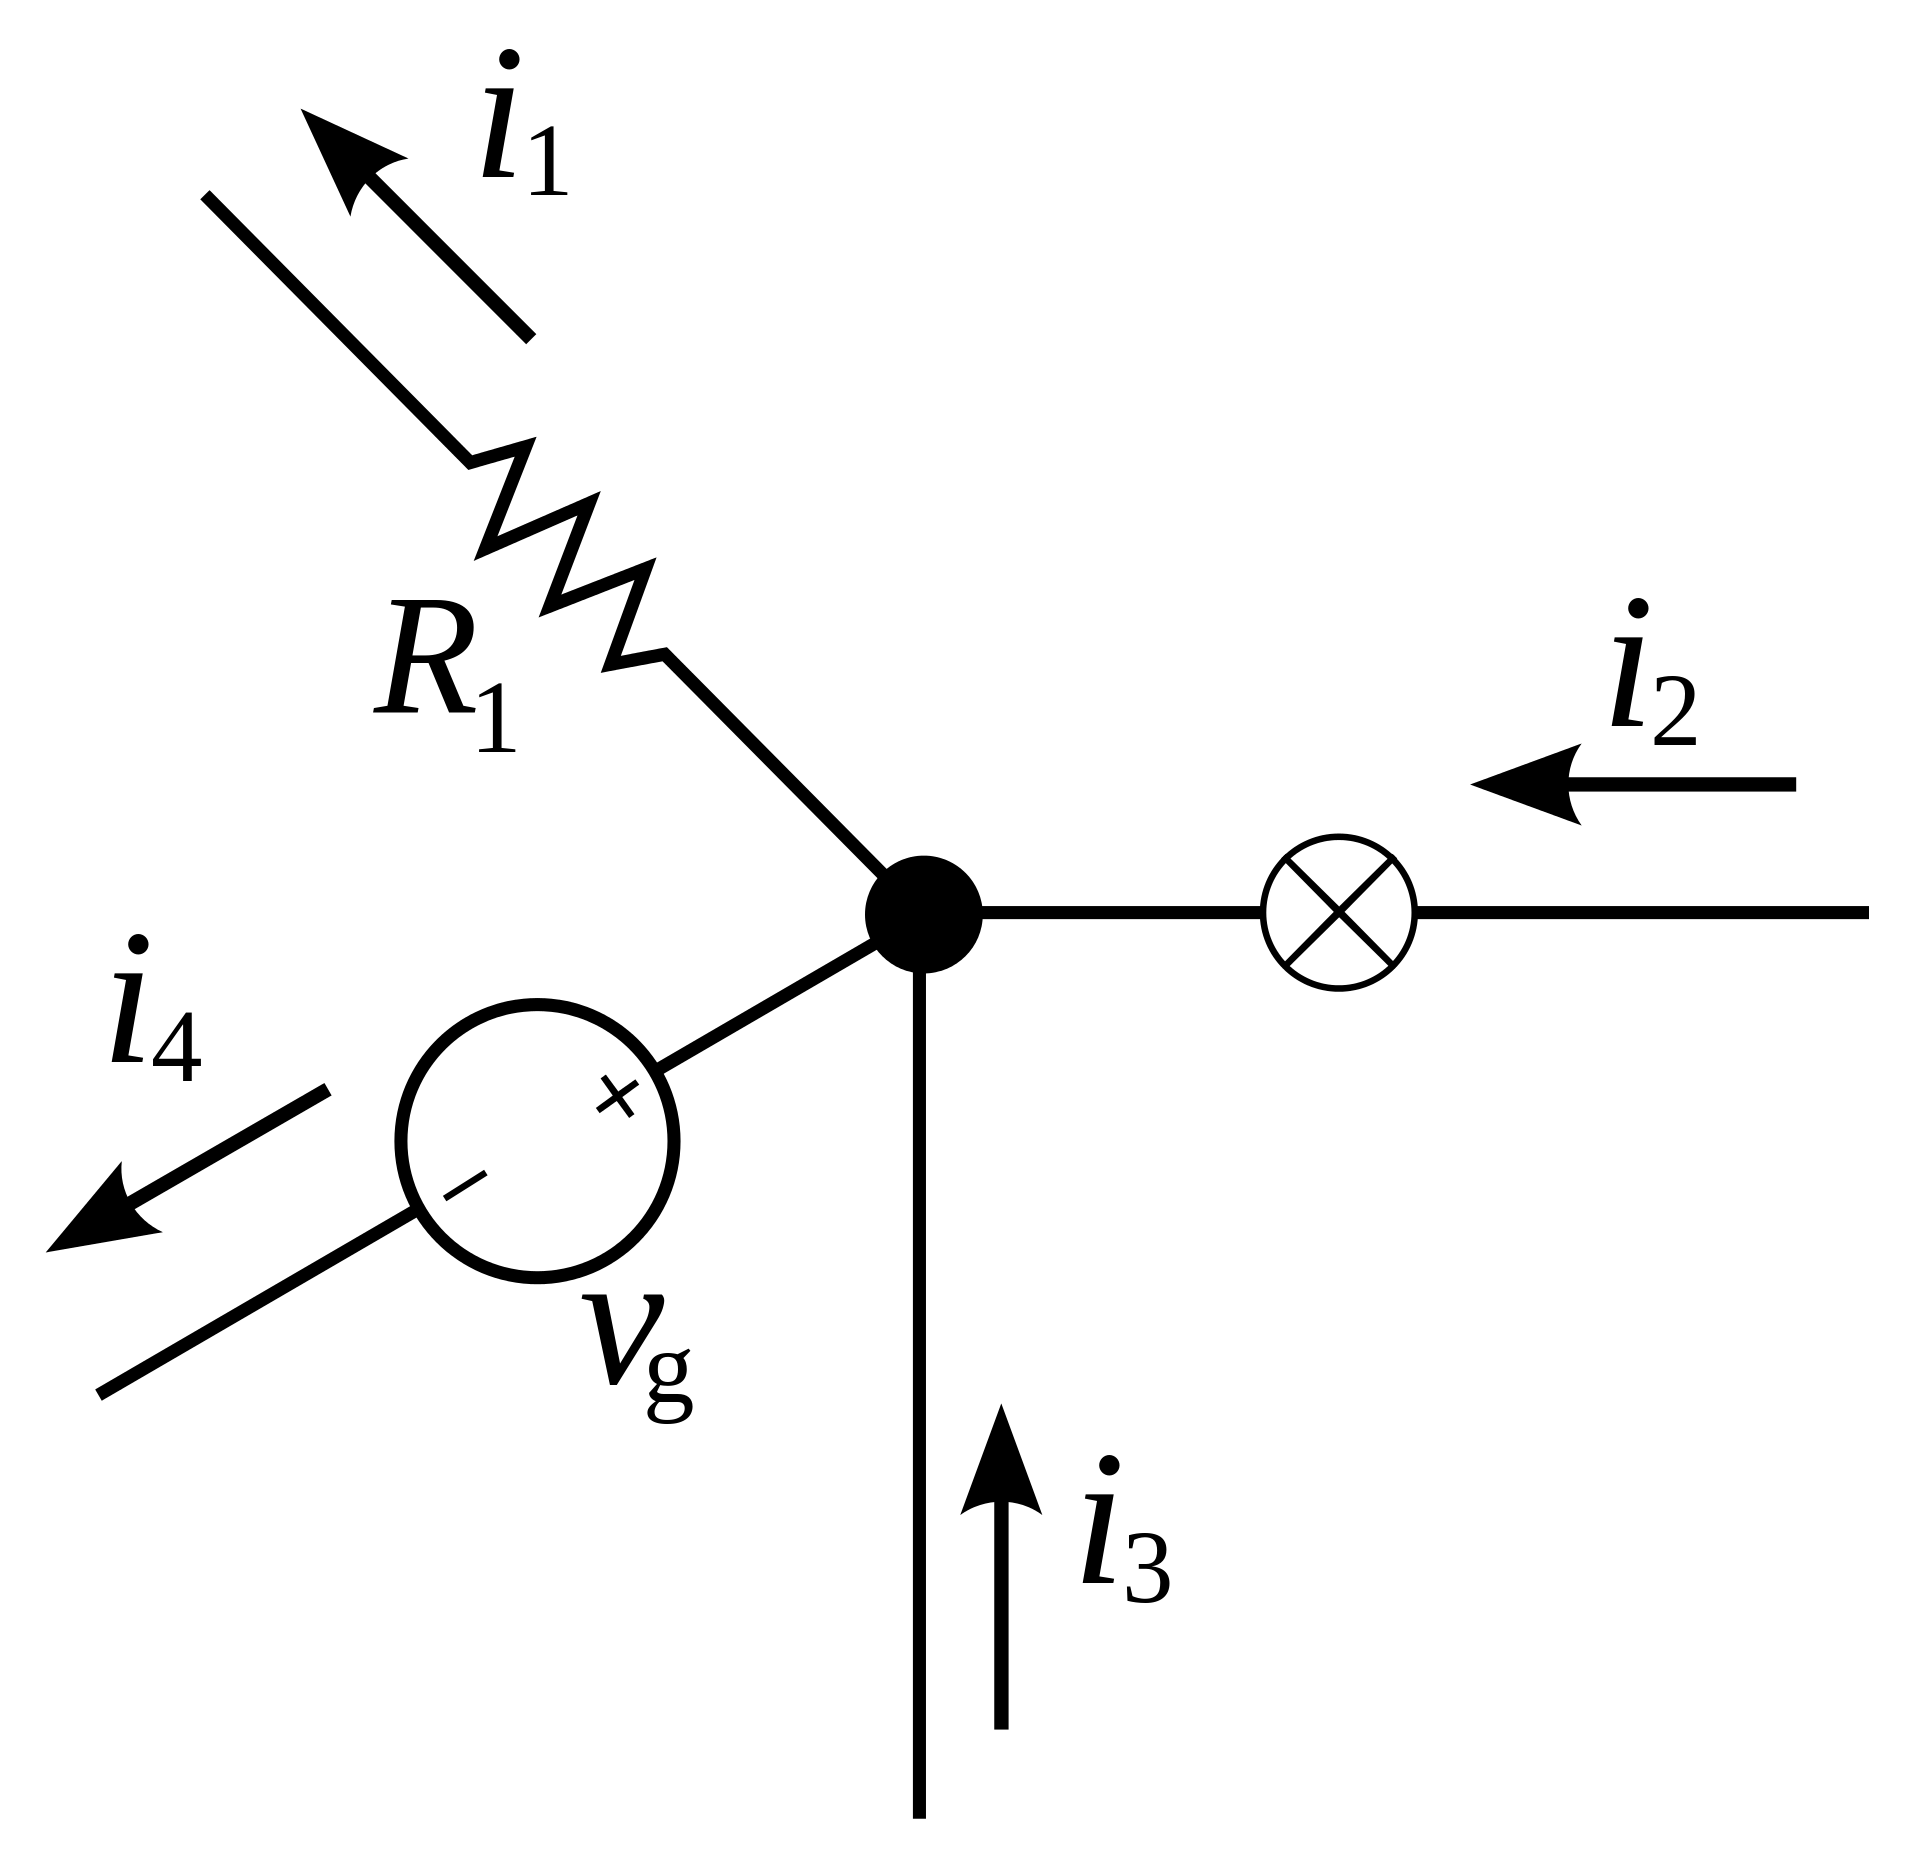
\includegraphics[width=5cm, center]{kirchoff1}

Matematikai képlettel kifejezve:
\begin{equation}
    \sum_{n} I_n = 0
\end{equation}

\section{Kirchoff II. törvénye: a huroktörvény}
A törvény értelmében bármely zárt hurokban a feszültségek előjeles összege nulla.

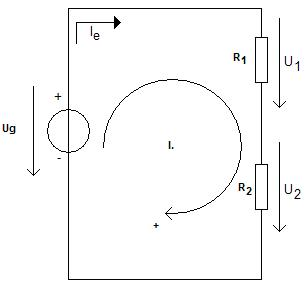
\includegraphics[width=5cm, center]{kirchoff2}

Matematikai képlettel kifejezve:
\begin{equation}
    \sum_{n} U_n = 0
\end{equation}

\section{Kirchhoff-törvények alkalmazása}
A fentebb ismertetett három törvény: az Ohm törvény, valamint Kirchhoff I. és II. törvénye a villamos hálózatokkal kapcsolatos számítások három alaptörvénye. Ezek a törvények biztosítják a szükséges eszközöket az elektromos áramkörök összetett viselkedésének elemzéséhez és megértéséhez. Alkalmazásuk széles körű, beleértve az áramköri tervezést, hibaelhárítást és az elektronikai eszközök fejlesztését is.

\end{document}
